\begin{enumerate}

\item[a)]Definimos las entradas 13 (tarea inicial), 14 (tarea idle), 15-22 (tareas jugador 1), 23-30 (tareas jugador 2) de la GDT
A estas entradas se les asigna tipo 9 (Execute-Only,accessed), base 0, presente 1 y DPL 0. El límite se establece en {\tt 0x68} para que sea mayor al tamaño de una TSS. La Figura \ref{fig:gdt2} muestra el estado de la GDT luego de agregar estas entradas.

\begin{figure}[h]
	  \centering
	    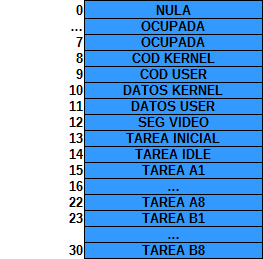
\includegraphics[ width=0.25\textwidth]{imagenes/gdt final.png}
	     \caption{Estado final de la GDT}
	  \label{fig:gdt2}
%	  \vspace{-15pt}
	\end{figure}
%	\FloatBarrier

\item[b)]Para completar la TSS de la tarea Idle hacemos uso de la función {\tt tss\_inicializar\_tarea\_idle}, la cual se encarga de asignar los segmentos de datos del kernel a los campos GS, FS, DS, SS, ES y poner el segmento de código de kernel en el campo CS. A su vez, completa ESP y EBP con la dirección del stack del kernel y se ocupa de que comparta el cr3 con el kernel. Por último, el EIP será {\tt 0x16000}, el campo EFLAGS se completa con {\tt 0x202} (para habilitar las interrupciones), el IOMAP con {\tt 0xFFFF} y el resto se deja en 0.

\item[c)] La función {\tt tss\_inicializar\_tareas\_piratas} toma como parámetro un puntero a tss y se ocupa de llenar sus campos. Los campos ES, SS, DS, FS y GS se completan con el segmento de datos de usuario, y el campo CS se completa con el segmento de código de usuario. Tanto ESP como EBP quedan seteados en {\tt 0x401000}, el campo EFLAGS en {\tt 0x202}, el CR3 en 0 (se le asignará un cr3 al momento de lanzar el pirata correspondiente utilizando la función {\tt mmu_inicializar_dir_tarea}), se pedirá una página nueva para el ESP0, SS0 se completa con segmento de datos kernel, IOMAP con {\tt 0xffff} y el resto con 0. 

\item[d)] En la rutina {\tt tss\_inicializar} pedimos una página libre para la tss de la tarea inical y asignamos la dirección obtenida en el campo {\it base} de la entrada correspondiente a esta tarea en la GDT.

\item[e)] En la rutina {\tt tss\_inicializar} completamos la entrada de la GDT perteneciente a la tarea Idle, completando el campo {\it base} con la dirección correspondiente a la misma.

\item[f)]Para pasar a la tarea IDLE primero se carga la tarea inicial en {\tt kernel.asm}, haciendo uso de la instruccion {\tt ltr} y de la dirección del segmento de la tss inicial. Una vez cargada la tarea inicial, se ejecuta un {\tt jmp} a la etiqueta seg_tss_idle, que corresponde al segmento de la tss Idle.

\begin{lstlisting}[frame=single]
%define selector_Inicial 0x0068 ;0000000001101011
%define selector_Idle 0x070 ;0000 0000 0111 0011

...

; Cargar tarea inicial
mov ax, selector_Inicial
ltr ax

; Saltar a la primera tarea: Idle
jmp selector_Idle:0

...
\end{lstlisting}

\item[g)]

\item[h)]Para este apartado hicimos algo más que lo pedido por el enunciado. Probamos lanzar una tarea explorador a través los siguientes pasos: llamar a {\tt inic_game} (función que se encarga de inicializar las variables globales del juego como los jugadores con sus respectivos puertos, 0 tareas activas, etc y todas las tareas piratas correspondientes a cada jugador como muertas y con sus respectivos indices, entre otras cosas), luego, mediante {\tt tss_inicializar} realizamos lo concerniente a la tss de las tareas (dejando lugar para un cr3 que se creara luego), y para finalizar ya dentro del juego presionamos la tecla RSHIFT (cual shift se presiona resulta indiferente para los efectos de la prueba). Presionando RSHIFT se llama a {\tt game_lanzar_pirata} que se encarga de inicializar el mapa de memoria de la tarea, copiar su codigo en el mapa y completar su campo posicion, además de mostrarla en el mapa de juego. Por último se procede a correr esa tarea previamente lanzada.
